% ============================================================
%  03_entree_dual.tex — Section 3 : du benzenoide au graphe dual
% ============================================================
\section{Traitement de l'entrée : du benzénoïde au graphe dual}

\subsection{Exemple fil rouge : \texttt{first.graph}}

L'exemple utilisé tout au long de cette section est un benzénoïde linéaire à 3 hexagones
(14 carbones), illustré ci-dessous. Les hexagones sont numérotés $v_0$, $v_1$, $v_2$.

\begin{center}
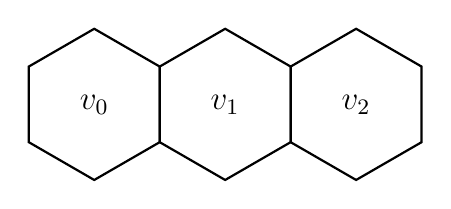
\begin{tikzpicture}[scale=0.8, every node/.style={font=\large}]
  % Hexagone v0
  \foreach \i in {0,...,5} {
    \coordinate (A\i) at ({cos(60*\i+30)*1.2}, {sin(60*\i+30)*1.2});
  }
  \draw[thick] (A0) -- (A1) -- (A2) -- (A3) -- (A4) -- (A5) -- cycle;
  \node at (0,0) {$v_0$};
  % Hexagone v1 (decale a droite)
  \foreach \i in {0,...,5} {
    \coordinate (B\i) at ({cos(60*\i+30)*1.2 + 2*1.2*cos(30)}, {sin(60*\i+30)*1.2});
  }
  \draw[thick] (B0) -- (B1) -- (B2) -- (B3) -- (B4) -- (B5) -- cycle;
  \node at ({2*1.2*cos(30)},0) {$v_1$};
  % Hexagone v2 (decale a droite x2)
  \foreach \i in {0,...,5} {
    \coordinate (C\i) at ({cos(60*\i+30)*1.2 + 4*1.2*cos(30)}, {sin(60*\i+30)*1.2});
  }
  \draw[thick] (C0) -- (C1) -- (C2) -- (C3) -- (C4) -- (C5) -- cycle;
  \node at ({4*1.2*cos(30)},0) {$v_2$};
\end{tikzpicture}
\end{center}

Le graphe dual correspondant est le chemin $v_0 - v_1 - v_2$ (deux arêtes).

\subsection{Format d'entrée Benzai}

Le fichier \texttt{.graph} utilise un format inspiré de DIMACS. Voici l'exemple
\texttt{first.graph} (3 hexagones linéaires, 14 carbones) :

\begin{lstlisting}[style=benzai]
p DIMACS 14 16 3
e 0_0 1_1
e 0_0 -1_1
e 1_1 1_2
e -1_1 -1_2
e 1_2 0_3
...
h 0_0 1_1 1_2 0_3 -1_2 -1_1
h -1_2 0_3 0_4 -1_5 -2_4 -2_3
h -2_4 -1_5 -1_6 -2_7 -3_6 -3_5
\end{lstlisting}

\begin{itemize}
  \item \texttt{p DIMACS V E F} : en-tête avec $V$ sommets (carbones), $E$ arêtes (liaisons)
    et $F$ faces (hexagones).
  \item \texttt{e s1 s2} : arête entre les carbones \texttt{s1} et \texttt{s2}. Les identifiants
    sont des coordonnées du réseau hexagonal (\texttt{x\_y}).
  \item \texttt{h s1 s2 s3 s4 s5 s6} : hexagone défini par ses 6 sommets dans l'ordre
    cyclique.
\end{itemize}

\subsection{Construction du graphe dual $\GD$}

Le \textbf{graphe dual} est la structure centrale du modèle CSP. Chaque hexagone du benzénoïde
devient un \textbf{sommet} du dual, et deux sommets du dual sont reliés par une arête si les
hexagones correspondants \textbf{partagent un côté}.

\begin{definition}[Graphe dual]
  Soit $\mathcal{B}$ un benzénoïde à $h$ hexagones. Le graphe dual
  $\GD = (V_D, E_D)$ est défini par :
  \begin{itemize}
    \item $V_D = \{0, 1, \ldots, h-1\}$ (un sommet par hexagone)
    \item $(u, v) \in E_D$ ssi les hexagones $u$ et $v$ partagent une arête
  \end{itemize}
\end{definition}

L'implémentation utilise NetworkX :

\begin{lstlisting}
# Construction du graphe dual (parser.py)
# hex_edges[u] = ensemble des aretes de l'hexagone u
for u in range(h):
    for v in range(u + 1, h):
        shared = hex_edges[u] & hex_edges[v]
        if shared:
            graph.dual.add_edge(u, v)
            # Enregistrer la position de l'arete partagee
            shared_edge = next(iter(shared))
            s1, s2 = tuple(shared_edge)
            pos_u = _find_edge_position(hexagons[u], s1, s2)
            pos_v = _find_edge_position(hexagons[v], s1, s2)
            graph.edge_positions[(u, v)] = (pos_u, pos_v)
\end{lstlisting}

\subsection{Motif d'occupation $\sigma(v)$}

Pour chaque hexagone $v$, le \textbf{motif d'occupation} (ou \textit{pattern})
$\sigma(v) \in \{0, 1\}^6$ indique quels côtés sont partagés avec un voisin dans le dual.
C'est un masque binaire qui décrit la ``forme'' du voisinage de l'hexagone.

\begin{definition}[Motif d'occupation]
  $\sigma(v) = (\sigma_0, \sigma_1, \ldots, \sigma_5)$ où $\sigma_i = 1$ si le côté $i$
  de l'hexagone $v$ est partagé avec un hexagone voisin, et $\sigma_i = 0$ sinon.
\end{definition}

\begin{lstlisting}
# Calcul des patrons (parser.py)
for v in range(h):
    pattern = [0] * 6
    for u in graph.dual.neighbors(v):
        pos = graph.edge_positions[(v, u)][0]
        pattern[pos] = 1
    graph.patterns[v] = tuple(pattern)
\end{lstlisting}

\textbf{Exemple} pour \texttt{first.graph} (3 hexagones linéaires) :
\begin{center}
\begin{tabular}{ccl}
  \toprule
  Hexagone & Degré & Patron $\sigma(v)$ \\
  \midrule
  $v_0$ & 1 & $(0, 0, 0, 1, 0, 0)$ \\
  $v_1$ & 2 & $(1, 0, 0, 1, 0, 0)$ \\
  $v_2$ & 1 & $(1, 0, 0, 0, 0, 0)$ \\
  \bottomrule
\end{tabular}
\end{center}

\subsection{Comptage des blocs de zéros $b(v)$}

Le nombre de \textbf{blocs de 0 consécutifs} dans le motif cyclique détermine si un hexagone
est gelé (ne peut pas changer de taille).

\begin{lstlisting}
def count_zero_blocks(pattern):
    # Trouver un 1 comme point de depart
    start = next(i for i, p in enumerate(pattern) if p == 1)
    blocks, in_zero = 0, False
    for offset in range(len(pattern)):
        idx = (start + offset) % len(pattern)
        if pattern[idx] == 0:
            if not in_zero:
                blocks += 1
                in_zero = True
        else:
            in_zero = False
    return blocks
\end{lstlisting}

Si $b(v) \geq 2$, l'hexagone $v$ est \textbf{gelé} : ses côtés partagés ne forment pas un
bloc consécutif unique, et il est impossible de redimensionner le cycle en préservant les
arêtes partagées.
